\part{Mental Representation \& Conceptual Models}
\frame{\partpage}

\begin{frame}{Learning Outcomes}
	In this section you will learn how to...
	
	\begin{itemize}
		\item \textbf{Define} what is meant by the term `mental model'
		\item \textbf{Explain} the place of mental models in HCI
		\item \textbf{Explain} what a metaphor is
		\item \textbf{Describe} the use of metaphor in HCI
		\item \textbf{Describe} the use of mental models in HCI
	\end{itemize}
\end{frame}

\begin{frame}{Further Reading}
	\begin{itemize}
		\item Lackoff, G. and Johnson, M. (1980) \textit{Metaphors We Live By}. UCP.
		\item Norman, D. and Draper, S. (1986) \textit{User-Centred Systems Design: New Perspectives on Human-Computer Interaction}. LEA.
		\item Norman, D. (1983) `Some Observations on Mental Models' in Gentner and Stevens (eds) \textit{User-Centred Systems Design: New Perspectives on Human-Computer
		 Interaction}. Erlbaum.
		 \item Kempton, W. (1986) \textit{Two Theories of Home Heat Control}, Cognitive Science 10, pp. 75 - 90.
	\end{itemize}
\end{frame}

\begin{frame}{Mental Representation \& Conceptual Models}
	\begin{itemize}
		\item The ways in which information we see, hear, and feel is represented in our brains can have implications for design.
		\item Psychologists believe information is stored so it can be recalled readily.
		\item Topics on knowledge representation include semantic networks, scripts, mental models, and so on---a vast field.
		\item We can leverage these representations through the application of metaphors and conceptual models in designs.
	\end{itemize}
\end{frame}


\begin{frame}{Human Memory Storage}
	\begin{itemize}
		\item Attention and memory are linked --- you remember what you pay attention to (Perry, 2006).
		\item There are three forms of memory store to consider:
		\begin{itemize}
			\item \textbf{very short term sensory store}: iconic; echoic; haptic.
			\item \textbf{mid-term working memory}: commonly referred to as short-term memory.
			\item \textbf{long-term memory}: persistant storage of throughts and ideas.
		\end{itemize}
	\end{itemize}
\end{frame}

\begin{frame}{Human Memory Storage}
	\begin{itemize}
		\item Information moves through sensory to working memory through our attending to it.
		\item Information moves through working memory through rehersal.
	\end{itemize}
\end{frame}

\begin{frame}[fragile]{Socrative \texttt{JBYPC3BBY}}
	\begin{itemize}
		\item In pairs.
		\item An example of long-term memory use in an RTS is remember unit capabilities, while echoic memory might be a confirmation beep when issuing a command.
		\item Quietly discuss other ways we may use memory in an RTS game.
		\item \textbf{Explain ONE} key design decision.
	\end{itemize}
\end{frame}

\begin{frame}{Human Memory Storage}
	There are two sorts of memory usage which we can consider:

	\begin{itemize}
		\item \textbf{recognition}: cues in the environment remind us of things
		\item \textbf{recall}: drawing things from memory without a prompt
	\end{itemize}
\end{frame}

\begin{frame}{Human Memory Storage}
	People find recall more challenging than recognition. Normall (1888) calls these two uses of memory `knowledge in the head' and
	`knowledge in the world', with implications for the ways we use such knowledge:

	\begin{itemize}
		\item as internal representatons (human memory)
		\item from the world through external presentations (memos, events)
		\item embodied in constraints from the world (the limits imposed on our behaviours from the environment
	\end{itemize}
\end{frame}

\begin{frame}[fragile]{Socrative \texttt{JBYPC3BBY}}
	\begin{itemize}
		\item In pairs.
		\item An example of `knowledge in the world' are greyed-out menu items --- users recognise they are not available and do not need to recall this.
		\item Quietly discuss other examples of `knowledge in the world' expressed in a game interface.
		\item \textbf{State ONE} example.
	\end{itemize}
\end{frame}

\begin{frame}{Human Memory Storage}
	Good game interfaces emphasise recognition and knowledge in the world over recall and knowledge in the head.
\end{frame}

\begin{frame}{A Cognitive Economy}
	Nonetheless, there are ways we can improve recall where it is neccessary. Knowledge is organised by people to promote a cognitive economy (Collins \& Quillan, 1969); 
	we do not conduct exhaustive searches of our memory every time we wish to recall something. It is organised in some way.
\end{frame}

\begin{frame}{A Cognitive Economy}
	Two such examples include:

	\begin{itemize}
		\item \textbf{semantic networks}: knowledge is organised by association.
		\item \textbf{scripts}: an encoding of knowledge about a particular context, such that it can guide behaviour.
	\end{itemize}
\end{frame}

\begin{frame}[fragile]{Socrative \texttt{JBYPC3BBY}}
	\begin{itemize}
		\item In pairs.
		\item An example of a semantic network in action is knowing the capabilities of a character based on its class (e.g. a cleric and monk are healers).
		\item An example of a script is knowing what to do to recruit a pick-up group in an MMORPG.
		\item Quietly discuss how semantics and scripts may influence game interaction.
		\item \textbf{Explain ONE} example, \textbf{briefly stating} which concept you are referring to.
	\end{itemize}
\end{frame}

\begin{frame}{Mental Models in Psychology}
	\begin{itemize}
		\item Norman (1983) describes mental models as `mental simulations'; models that people have of themselves, others,the environment, things they interact with, etc.
		\item Remember the fridge example from last week? You may well have developed an incorect mental model while trying to decipher the controls.
	\end{itemize}
\end{frame}

\begin{frame}{Mental Models in Psychology}
	\begin{centering}
		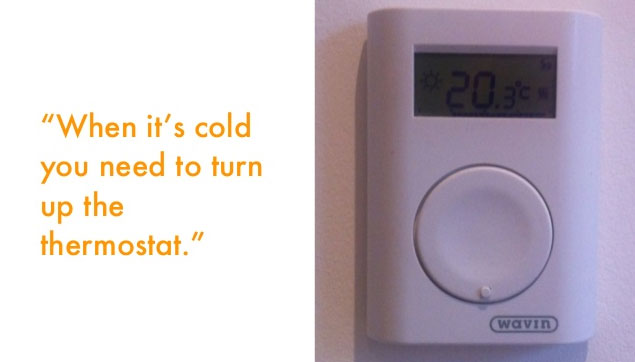
\includegraphics[height=26ex]{thermostat_invalid_model.jpg}
	\end{centering}
	
	\vspace{2ex}
	
	(see Kempton, 1986)
\end{frame}


\begin{frame}[fragile]{Socrative \texttt{JBYPC3BBY}}
	\begin{itemize}
		\item Briefly, is the statement correct?
	\end{itemize}
\end{frame}

\begin{frame}{Mental Models in Psychology}
	\begin{itemize}
		\item We build mental models to predict external events before we take action.
		\item Play an important role in human reasoning, and consequently player behaviour in games.
		\item Are players developing an accurate mental model?
	\end{itemize}
\end{frame}

\begin{frame}{Mental Models in Psychology}
	\begin{centering}
		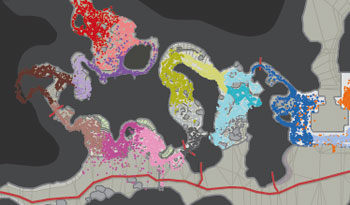
\includegraphics[height=20ex]{halo_heat_map.jpg}
	\end{centering}
	
	\vspace{2ex}
	
	(Thomson, 2007) \\
	\url{http://archive.wired.com/gaming/virtualworlds/magazine/15-09/ff_halo?currentPage=all}
\end{frame}

\begin{frame}{Conceptual Models in the Interface}
	\begin{itemize}
		\item Players need to understand their actions in order to make meaningful choices.
		\item As such, designers need to design an interface in a way that shapes the players' mental model construction.
		\item Normal (1988) suggests how the design and the player's mental model are linked through the `system image' (i.e. the visible part
		of the interactive system).
	\end{itemize}
\end{frame}

\begin{frame}{Conceptual Models in the Interface}
	``In many ways the primary task of designer is to construct an appropriate system image, realising that everything the user interacts with helps us to inform that image:
	the physical knobs, dials, keyboards, and displays [...] text, input, output, and error messages''
	
	\vspace{2ex}
	
	(Normal, 1986, p. 44)
\end{frame}

\begin{frame}{Conceptual Models in the Interface}
	Newman and Lamming (1995) provide design guidelines along these lines:

	\begin{itemize}
		\item Identify the mental model you intend the player to adopt, preferably before designing the game interface;
		\item Link the mental model to the intended means of interaction;
		\item Hide aspects of the system image that conflict with player performance on an action/activity;
		\item Explout the system image to convey the intended mental model;
		\item and show the state of the game as it is \textit{now}---not as it was some time ago.
	\end{itemize}
\end{frame}